\documentclass[tikz,border=3pt]{standalone}
\usepackage{xcolor}
\usetikzlibrary{decorations.pathreplacing,positioning}
\definecolor{waveorange}{HTML}{EA580C}
\definecolor{devicegray}{HTML}{475569}
\definecolor{devicefill}{HTML}{F8FAFC}
\begin{document}
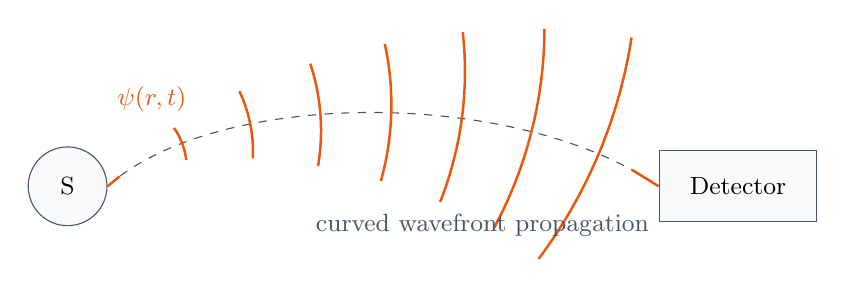
\begin{tikzpicture}[every node/.style={font=\small}]
  \node[draw=devicegray,fill=devicefill,circle,minimum size=10mm] (emitter) {S};
  \node[draw=devicegray,fill=devicefill,minimum width=2cm,minimum height=9mm,
    right=7cm of emitter] (sensor) {Detector};
  \draw[devicegray,dashed]
    (emitter.east) .. controls +(1.4,1.25) and +(-1.8,1.25) .. (sensor.west);
  \draw[waveorange,line width=.9pt,decorate,
    decoration={expanding waves,segment length=9mm,angle=14,
      pre length=2mm,post length=4mm}]
    (emitter.east) .. controls +(1.4,1.25) and +(-1.8,1.25) .. (sensor.west);
  \node[waveorange,above=11mm of emitter.east,anchor=west] {$\psi(r,t)$};
  \node[devicegray,below=5mm of sensor.west,anchor=east] {curved wavefront propagation};
\end{tikzpicture}
\end{document}
